\chapter{Milestone 5}
\section{Berendsen Thermostat Teststrategy}
\begin{comment}
-basic idea is weather or not the implementation follows the exponential damping from the 2 equation for a small system with known velocities
\end{comment}
%equations
\begin{equation}
	\lambda = \sqrt{1 + \bigg(\frac{T_{0}}{T} -1\bigg)\frac{\Delta t}{\tau}}
\end{equation}

\begin{equation}
	T(t) = T_{0} + (T_{1}-T_{0})e^{-t/\tau}
\end{equation}

\section{Simulation Time}
\begin{comment}
simulation should be roughly of complexity N2
may need too approximate with a function 
\end{comment}
\begin{figure}[!h]
	\begin{center}
		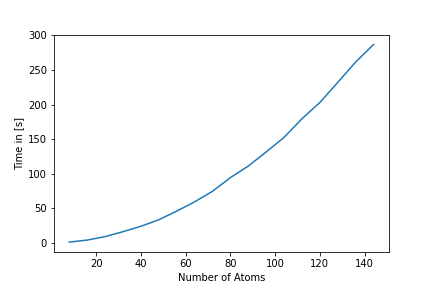
\includegraphics[scale=1]{Figure/plotAtomTimes.png}
	\end{center}
	\caption[Simulationtime]{Simulationtime from 8 to 192 Atoms }
	\label{PlotAtomTimes}
\end{figure}


